\documentclass[10pt,a4paper,twocolumn]{article}

\usepackage[T1]{fontenc}
\usepackage[sc]{mathpazo}
\usepackage[scale=0.92]{tgheros}
\usepackage[a4paper,margin=19mm,headsep=5mm,footskip=10mm]{geometry}
\usepackage{microtype}
\usepackage{amsmath,amssymb,amsthm}
\usepackage{algorithm,algpseudocode}
\usepackage{booktabs,graphicx}
\usepackage{xcolor,titlesec}
\usepackage{tikz}
\usetikzlibrary{arrows.meta,positioning}
\usepackage[round,sort]{natbib}

\definecolor{Ink}{HTML}{1F303B}
\definecolor{ProjectBlue}{HTML}{174F91}
\definecolor{ReferenceTeal}{HTML}{14675A}
\definecolor{LinkSlate}{HTML}{314E67}
\usepackage[colorlinks=true,urlcolor=ProjectBlue,citecolor=ReferenceTeal,
  linkcolor=LinkSlate,pdfborder={0 0 0},
  pdftitle={Weather Chronology and Green Hydrogen Reliability},
  pdfauthor={Parsa Besharat},
  pdfsubject={A reproducible climate-to-hydrogen storage pilot near Syracuse, New York}]{hyperref}

\setlength{\columnsep}{7mm}
\setlength{\emergencystretch}{1.3em}
\setlength{\bibsep}{4pt}
\widowpenalty=10000
\clubpenalty=10000
\raggedbottom
\titleformat{\section}{\large\sffamily\bfseries\color{Ink}}{\thesection}{0.65em}{}
\titleformat{\subsection}{\normalsize\sffamily\bfseries\color{Ink}}{\thesubsection}{0.6em}{}
\newtheorem{proposition}{Proposition}[section]
\newcommand{\RepoURL}{https://github.com/parsabe/Beyond-Normal-Weather}
\newcommand{\RepoRoot}{\href{\RepoURL}{GitHub repository}}
\newcommand{\RepoPipeline}{\href{\RepoURL/tree/hydrogen-pipeline}{pipeline code}}
\newcommand{\RepoBenchmarks}{\href{\RepoURL/tree/hydrogen-benchmarks/reports}{benchmark results}}
\newcommand{\CRPS}{\operatorname{CRPS}}
\newcommand{\clip}{\operatorname{clip}}
\providecommand{\doi}[1]{\href{https://doi.org/#1}{\nolinkurl{#1}}}

\title{\bfseries\color{Ink} Weather Chronology and Green Hydrogen Reliability\\[3pt]
  \large\normalfont A storage-calibrated downscaling pilot near Syracuse, New York}
\author{Parsa Besharat\\[-1pt]\normalsize\href{mailto:parsa@parsabe.com}{\texttt{parsa@parsabe.com}}}
\date{}

\begin{document}
\maketitle

\begin{abstract}
Wind and solar droughts can interrupt delivery from an off-grid hydrogen plant when low generation persists long enough to empty its storage tank. Climate projections provide daily weather sequences, but local bias correction and chronological post-processing can change the clusters of low production that drive such shortages. This pilot asks whether the dependence model can be calibrated against hydrogen delivery outcomes while holding the corrected monthly wind and solar distributions fixed. Hourly ERA5 reanalysis defines local generation proxies for an illustrative plant near Syracuse, New York. Daily output from three CMIP6 models is corrected using monthly additive quantile delta mapping, then reordered with paired historical rank blocks. The block length and replacement probability are selected using the continuous ranked probability score for annual unmet demand across four tank sizes. The selected three-day blocks reduced mean calibration CRPS from 0.628 to 0.572 percentage points. Climate-model chronology scored better on the eight withheld years at all five tested tank sizes, including the seven-day tank excluded from tuning, where CRPS was 0.477 versus 0.548 percentage points. Timing still mattered for projected shortages. Under SSP2-4.5, paired-day shuffling lowered mean unmet demand from 2.28\% to 1.47\% for a three-day tank. In an external comparison against a published grid cell, storage-calibrated resampling brought the projected increase in flash wind drought frequency closer to the published estimate, while solar changes varied across models. These results support using climate-model order as the reference for this site and explicitly testing how chronology choices affect storage conclusions. Reproduction materials are available in the \RepoRoot, with the \RepoPipeline\ and \RepoBenchmarks.
\end{abstract}

\section{Introduction}
\label{sec:introduction}
An electrolyzer supplied by wind and solar generation can continue serving a delivery contract after generation drops if its tank contains enough hydrogen. The sequence of weather therefore influences reliability through the inventory carried from one day to the next. Two periods with the same daily wind and solar pairs can lead to different shortages when low-generation days are concentrated in one period and separated by opportunities to refill the tank in the other. Persistent and temporally compounding weather conditions have been linked to long episodes of unmet demand in renewable electricity systems, and abrupt renewable drought onset can increase operational difficulties \citep{vandermost2024,lin2026}. Long-term hydrogen studies also show that location-specific wind and solar sequences are relevant to plant design and economics \citep{wu2026}. These findings motivate a local modeling problem. Global climate simulations represent the large-scale climate response, yet their daily resource distributions and weather dependence can differ from a local reanalysis. Correcting each variable's marginal distribution addresses one part of this mismatch. The wind--solar association and the ordering of low-generation days determine how much of that correction carries through to storage and delivery. This paper tests whether selecting a paired rank-block resampling rule on the distribution of plant shortfalls improves generalization across years and tank sizes. All chronology methods receive the same corrected monthly resource values, and all are evaluated through the same idealized plant. This design makes chronology the experimental change. A Syracuse case study compares the proposed rule with climate-model order and a fixed seven-day resampler, then perturbs persistence and wind--solar alignment in separate diagnostics. An external comparison applies published flash-drought thresholds and time windows to test whether conclusions about the weather hazard agree with the nearest published grid cell. Separating the historical test from method selection and reporting both operational skill and external hazard agreement allows either criterion to favor a different method.

\section{Related Work}
\label{sec:related}
\paragraph{Marginals and dependence.}
Quantile mapping adjusts biases in simulated weather distributions. When applied to a changing climate, conventional quantile mapping can modify modeled changes in the upper or lower tail. Quantile delta mapping incorporates the modeled change at each percentile \citep{cannon2015}. This study uses an additive correction for wind speed and downwelling shortwave radiation before a separate conversion to daily generation proxies. \citet{vrac2020} extend rank resampling to account for temporal dependence in multivariate climate bias correction. Their work motivates retaining paired, consecutive reference ranks. The procedure here uses a two-variable block library and chooses block settings through a downstream storage score. The historical test includes both the original model chronology and a fixed resampling rule to separate the value of tuning from the value of resampling itself.

\paragraph{Energy droughts and system operation.}
\citet{vandermost2024} show how weather and energy-system conditions can compound across time in European electricity systems with hydropower. \citet{lin2026} link abrupt and prolonged wind and solar droughts to electricity dispatch impacts and provide gridded projections of changes in event frequency. These studies support evaluating both the weather sequence and its consequences for the system. The present experiment fixes a hydrogen delivery contract and simulates an explicit tank with carryover. The Lin et al. comparison tests the weather hazard using the authors' published source workbook \citep{lin2026data}. It complements the storage test, which uses a mass-based hydrogen shortfall outcome.

\paragraph{Hydrogen under future climates.}
\citet{wu2026} estimate future costs and configurations across locations using hourly wind and solar capacity factors derived from eight CMIP6 models. Their optimization includes technology capacities and storage, whereas this study fixes plant and delivery assumptions and tests sensitivity to daily weather chronology. Their capacity-factor series are available from the corresponding author by request. The hourly optimization is therefore a related application, and the Lin et al. workbook supplies the downloadable reference for the numerical comparison reported here.

\section{Methodology}
\label{sec:methodology}
The pipeline separates the distribution of each resource from the sequence that reaches the plant. Figure~\ref{fig:workflow} in the appendix shows the data flow. First, local reanalysis supplies a weather and generation reference. Each climate model is mapped to this reference at the level of monthly distributions. The baseline retains climate-model day order after that mapping. The candidate changes the order and wind--solar pairing before applying the same daily dispatch model.

\subsection{Weather inputs and local capacity factors}
\label{sec:datasets}
The reference site is Syracuse, New York (43.05$^{\circ}$N, 76.15$^{\circ}$W). ERA5 provides hourly 10\,m and 100\,m wind speeds and surface downward shortwave radiation, accessed through the Open-Meteo archive \citep{hersbach2020,openmeteo}. For the wind proxy, a cubic power curve starts at 3\,m\,s$^{-1}$, reaches rated power at 12\,m\,s$^{-1}$, and switches off at 25\,m\,s$^{-1}$. For the solar proxy, hourly radiation in W\,m$^{-2}$ is multiplied by $0.85/1000$ and clipped to $[0,1]$. Averaging the resulting hourly capacity factors gives the daily generation reference. Daily 10\,m wind and shortwave radiation are also averaged for comparison with the global models. Radiation intervals are grouped by their reported UTC timestamp. The derived capacity factors represent an idealized system driven by reanalysis.

The CMIP6 inputs are daily near-surface wind speed and downward shortwave radiation from ACCESS-CM2, MPI-ESM1-2-HR, and MRI-ESM2-0 \citep{eyring2016,pangeo}. The pipeline selects the nearest native-grid point for each model and matches the model, realization, grid, and date between its two variables. Each model contributes one realization, \texttt{r1i1p1f1}. The source catalog records the version of each store. Extraction checks coverage, calendar, units, grid consistency, and daily continuity.

\subsection{Monthly marginal correction}
For a given model, calendar month, and resource, let $x_t$ be the target daily value and $q_t$ its empirical fractional rank within that calendar month across the target window. With average ranks for ties, $q_t=(\operatorname{rank}(x_t)-0.5)/n_m$, where $n_m$ is the number of target days in month group $m$. Write $Q_{R,m}$ for the ERA5 reference quantile function and $Q_{H,m}$ for the historical climate-model quantile function, both fitted on the training period. The correction takes the form
\begin{equation}
\label{eq:qdm}
\widetilde{x}_t = \max\!\left\{0,\,
  x_t+Q_{R,m}(q_t)-Q_{H,m}(q_t)\right\}.
\end{equation}
The implementation interpolates the quantile difference on 201 evenly spaced probability levels. The monthly generation transfer then interpolates from the ERA5 weather quantiles to the corresponding ERA5 capacity-factor quantiles and clamps outside the historical weather range. This use of additive quantile delta mapping carries modeled changes into the corrected weather values before nonnegative clipping and the nonlinear generation transfer. Both subsequent operations can attenuate changes in the tails. The resulting daily wind and solar capacity factors are common to all chronology methods for a given model and window.

\subsection{Conditional paired rank blocks}
Let $\mathbf{r}_t=(r_{t,w},r_{t,s})$ be the vector of monthly fractional ranks of the two corrected capacity factors. The scheme selects a block length $\ell$ and an independent block replacement probability $f$. Each member starts its partition at a random offset from $0$ through $\ell-1$. For an eligible start $t$, the method considers consecutive blocks in the ERA5 training archive that start in the same calendar month. It ranks candidate blocks by the sum of squared differences in the starting rank vector and the block-mean rank vector. The comparison uses the available target days at the end of a window. A selected replacement draws uniformly from the nearest 20 admissible source blocks, or all admissible blocks if fewer are available, and copies the paired ranks. The final target block receives only the needed prefix.

The resulting scores provide an order for the original corrected values. For each calendar month and each variable independently, the method assigns the sorted corrected values to the dates ordered by their resampled ranks. Stable ordering resolves ties. Each member thus preserves the exact empirical marginal distributions over all instances of a given calendar month in its window (Appendix~\ref{app:marginals}). Weather timing, same-day wind--solar pairing, and year-to-year concentrations can change. The model-order member corresponds to $f=0$. The fixed resampling comparison uses $(f,\ell)=(1,7)$, and a nonzero setting produces 24 sequences per model and window.

\subsection{Hydrogen dispatch and annual shortfall}
Let $w_t$ and $s_t$ denote daily capacity factors, $P_w$ and $P_s$ installed wind and solar power, and $P_e$ electrolyzer capacity, all power ratings in MW. With efficiency parameter $e$ in kWh per kg, produced hydrogen in kg is
\begin{equation}
\label{eq:production}
G_t = \frac{24{,}000}{e}\min\{P_e,\,P_ww_t+P_ss_t\}.
\end{equation}
Daily energy averaging places the electrolyzer cap on the daily equivalent power. Given contracted demand $D$ in kg per day, initial inventory $S_{t-1}$, and a tank of $k$ delivery days, the provisional balance $B_t$, unmet delivery $U_t$, and closing inventory $S_t$ are
\begin{equation}
\label{eq:dispatch}
\begin{aligned}
B_t &= S_{t-1}+G_t-D,\\
U_t &= \max\{-B_t,0\},\\
S_t &= \clip(B_t,0,kD).
\end{aligned}
\end{equation}
The plant serves delivery before storing surplus. Each sequence starts empty and repeats its first year once as warm-up before scoring. Inventory carries across scored years. The annual unmet share is $L_{y,k}=\sum_{t\in y}U_t/(D\,n_y)$, where $n_y$ is the number of days in the model's calendar year. The same dispatch and plant parameters are used for the ERA5 reference. Appendix~\ref{app:dispatch} proves mass balance and monotonicity with tank size for a fixed sequence.

\subsection{Storage-oriented model selection}
The score compares a simulated distribution of annual unmet demand at each tank size with each reference year. For $M$ simulated annual losses $z_1,\ldots,z_M$ and a reference loss $a$, the empirical continuous ranked probability score is
\begin{equation}
\label{eq:crps}
\begin{aligned}
\CRPS(\widehat F_M,a)
&=\frac{1}{M}\sum_{i=1}^{M}|z_i-a|\\[-2pt]
&\quad{}-\frac{1}{2M^2}\sum_{i,j=1}^{M}|z_i-z_j|.
\end{aligned}
\end{equation}
Lower values indicate better agreement between the predictive distribution and the reference \citep{gneiting2007}. The simulation pools annual losses from the three climate models, giving the models equal weight within each chronology method. The objective averages Eq.~\eqref{eq:crps} across ERA5 calibration years and tank sizes of 0, 1, 3, and 14 days. The search covers $f\in\{0.25,0.50,1\}$ and $\ell\in\{3,7,14\}$, plus the model-order baseline. The seven-day tank is excluded from selection. Appendix~\ref{app:crps} derives the equivalent sorted-sample expression used in the implementation.

\begin{algorithm}[t]
\caption{Fit and test the weather chronology}
\label{alg:pipeline}
\small
\begin{algorithmic}[1]
\Require ERA5, matched CMIP6 runs, plant, tank sizes
\Ensure Frozen block setting and shortfall distributions
\State Build daily ERA5 weather and generation proxies.
\State Fit monthly quantile maps on the training years.
\State Build a paired ERA5 rank library from those years.
\State Map each model's calibration weather to power.
\For{each candidate setting $(f,\ell)$}
  \For{each model and member}
    \State Partition the sequence into blocks of length $\ell$.
    \State Sample analog ranks with probability $f$ per block.
    \State Reorder corrected values by these monthly ranks.
    \State Dispatch the plant for each tuning tank size.
  \EndFor
  \State Pool model losses and score against ERA5 years.
\EndFor
\State Freeze the setting with the smallest mean CRPS.
\State Evaluate all methods on the withheld years and tank.
\State Apply frozen settings to the two future scenarios.
\end{algorithmic}
\end{algorithm}

\subsection{Sequence diagnostics}
Two interventions perturb the model-order sequence after marginal correction. One randomly permutes paired wind and solar days within each calendar month and year, preserving same-day resource pairs while weakening chronological runs. The other applies a random circular shift to solar within each month and year, leaving the wind series intact and largely preserving solar runs within the month apart from the wrap. It changes wind--solar alignment. Both conserve each resource's values within each month and year. Edges between shifted months and the reordering itself limit interpretation as single-mechanism physical interventions. Appendix~\ref{app:timing} gives a worked example of changed storage losses under an exact permutation of production values.

\section{Experiments}
\label{sec:experiments}

\subsection{Study design and historical test}
The illustrative off-grid plant has 30\,MW of wind capacity, 20\,MW of solar capacity, and a 25\,MW electrolyzer using 52\,kWh per kilogram of hydrogen. The delivery contract is 2{,}700\,kg per day. Tested tank sizes hold 0, 1, 3, 7, or 14 days of contracted demand. This design keeps production, dispatch rules, and demand fixed across scenarios. It excludes grid imports, inventory losses, and intra-day operating constraints.

ERA5 and historical CMIP6 data from 1981--1998 train the marginal maps and supply reference analog blocks. The 1999--2006 period is used to select the block parameters. Evaluation uses 2007--2014, including the seven-day tank excluded from selection. Climate simulations are free-running, so the comparison scores the distribution of annual outcomes against each reference year, with no day-by-day or year-by-year weather pairing. The model's fractional ranks for each evaluation period use only its own simulated resource values for that period. The held-out ERA5 primary data enter through the reference dispatch outcomes used for scoring.

We report the mean CRPS by tank size across the eight ERA5 test years. The number of climate and resampled trajectories describes the forecast distribution. The statistical comparison still has eight reference years. To illustrate sensitivity to that sample, we resample the paired annual score differences with circular two-year blocks over the withheld ERA5 years and use the 2.5th and 97.5th percentiles of 2{,}000 bootstrap averages. These bounds are conditional on the fitted settings and the pooled forecast distributions. They exclude uncertainty from other climate models, plant designs, and sites.

\subsection{Future scenarios and sequence interventions}
The historical choice of block length and replacement rate is frozen before application to 2041--2060 under SSP2-4.5 and SSP5-8.5. For every model and scenario, the pipeline reports mean and 90th-percentile annual unmet demand, the fraction of years above the shortfall target, the share of shortfall days, and the longest within-year run of unmet delivery. It also records the smallest tested tank for which average unmet demand is at most 1\%. We compare the two sequence interventions against the climate-model order under the same plant and weather inputs. Model spread is reported separately from resampling variability and scenarios are displayed individually.

\subsection{Published flash-drought comparison}
The weather-hazard comparison uses the Figure~2 source workbook and supplementary methods from \citet{lin2026}. The nearest eligible grid cell to the project site is 43.5$^{\circ}$N, 76.5$^{\circ}$W. We align SSP2-4.5, the historical window of 1985--2014, and the projection window of 2045--2074. In each historical trajectory, we identify complete spells of at least three days below the 10th-percentile capacity factor for each resource. The day-before drop defines onset speed. A flash drought has an onset above the 90th percentile of historical spell onsets. The future frequency is computed using the fixed thresholds from the corresponding historical trajectory. Spells touching either end of the window are excluded from the count.

The relative change is $100(\bar N_{\mathrm{future}}/\bar N_{\mathrm{hist}}-1)$, where $\bar N$ is the mean count per 30-year trajectory within model and method. Results are then averaged equally across models. A zero historical count makes the relative change undefined. The comparison uses the published grid cell as a numerical reference and preserves the separate scope of the hydrogen delivery experiment. The paper's model ensemble, grid resolution, and capacity-factor construction differ from those of this pilot.

\section{Results}
\label{sec:results}

\subsection{Historical pipeline evaluation}
Calibration selected $f=1$ and $\ell=3$, replacing every eligible block after the randomly chosen start offset. Averaged across the four tuning tank sizes, CRPS was 0.572 percentage points, compared with 0.628 for climate-model order. The next-best grid setting, a 50\% replacement rate with seven-day blocks, scored 0.576 percentage points. The small tuning difference between these two settings leaves room for instability in the selected parameters.

\begin{table}[t]
\centering\small
\caption{Mean test CRPS in percentage points for 2007--2014. Lower is better. The dagger marks the tank size withheld from model selection.}
\label{tab:test}
\begin{tabular}{@{}rrrr@{}}
\toprule
Tank days & Model order & Fixed blocks & Calibrated \\
\midrule
0 & \textbf{0.839} & 1.037 & 1.023 \\
1 & \textbf{0.622} & 1.184 & 1.023 \\
3 & \textbf{0.619} & 0.919 & 0.819 \\
7$^{\dagger}$ & \textbf{0.477} & 0.560 & 0.548 \\
14 & \textbf{0.0245} & 0.0245 & 0.0248 \\
\bottomrule
\end{tabular}
\end{table}

Climate-model order achieved lower CRPS than storage-calibrated resampling at every tested tank size in 2007--2014 (Table~\ref{tab:test}). For the held-out seven-day tank, calibrated CRPS exceeded the model-order score by 0.071 percentage points. The conditional moving-block bootstrap bounds were $-0.002$ and $+0.150$ percentage points. At 14 days the model-order and fixed-block scores agree to the displayed precision, and the calibrated score was slightly higher. These results favor the climate-model order for this pilot, while the short evaluation window limits broader claims about the relative skill of the methods.

\subsection{Projected delivery and chronology sensitivity}
Under climate-model order, the three-model mean unmet demand in 2041--2060 for a seven-day tank was 0.55\% under SSP2-4.5 and 0.60\% under SSP5-8.5. Storage-calibrated resampling gave 0.41\% and 0.48\%, respectively. Under the calibrated method, a seven-day tank was the smallest tested capacity meeting the 1\% mean shortfall target for all three models and both scenarios. With climate-model order, ACCESS-CM2 under SSP5-8.5 first met the target at 14 days, while the other model--scenario combinations met it at seven days. These capacities are grid-search results for an illustrative system and a period-average target. Appendix Figure~\ref{fig:hydrogen} shows the historical skill and future storage curves.

For three days of storage under SSP2-4.5, mean unmet demand reached 2.28\% under climate-model order. Paired-day shuffling lowered it to 1.47\%, even though each contemporaneous wind--solar pair was preserved within its month and year. Shifting solar alone raised it to 2.55\%. This pattern shows that the ordering of resource availability can materially affect delivery reliability for this plant. The shift experiment also changes the placement of month boundaries in the solar series, so its difference quantifies the full perturbation.

\subsection{Comparison with published drought data}
Table~\ref{tab:literature} compares the estimated changes in event frequency with the source grid cell from \citet{lin2026}. For wind, the calibrated estimate of $+16.4$\% is closer to the published value of $+11.8$\% than the model-order estimate of $+38.1$\%. Solar moves from $+63.2$\% with model order to $+9.1$\% with the calibrated method, while the published cell shows $-2.0$\%. Under calibrated resampling, the solar change ranges from $-52.3$\% to $+44.1$\% across the three climate models (Appendix Figure~\ref{fig:external}). Baseline historical counts for flash solar droughts are five to eight per model over 30 years, and small absolute changes can therefore move the relative frequency sharply.

\begin{table}[t]
\centering\small
\caption{Relative change in flash-drought frequency under SSP2-4.5. The published column uses the nearest eligible grid cell in the authors' Figure~2 workbook. Pilot columns are means across three climate models.}
\label{tab:literature}
\begin{tabular}{@{}lrrr@{}}
\toprule
Resource & Published & Model order & Calibrated \\
\midrule
Wind  & $+11.8$\% & $+38.1$\% & $+16.4$\% \\
Solar & $-2.0$\%  & $+63.2$\% & $+9.1$\% \\
\bottomrule
\end{tabular}
\end{table}

The external comparison evaluates one feature of the daily weather sequence across a different climate model ensemble and point-to-grid representation. It therefore complements the held-out test of annual hydrogen delivery. Agreement on the wind hazard and weaker test performance for storage coexist in this case. The benchmark branch preserves the weather event counts, the reference grid cell, and the input checksums. The \RepoBenchmarks\ contain both test outcomes.


\section{Future Work}
\label{sec:future}
The immediate test is whether storage-oriented calibration transfers across additional sites, model families, and weather periods. Rolling historical splits would provide more test windows, and a leave-one-model-family-out experiment could reveal how sensitive the estimated benefit is to each model's chronology. A nested evaluation would keep the held-out years entirely outside block design and selection. Score differences should be reported across the held-out cases, along with the number of reference drought events and a sensitivity analysis for the baseline windows. A stronger benchmark would acquire the plant-modeling study's hourly series and extend the published flash-drought comparison to matched model runs, locations, power conversions, and compound event definitions.

The candidate resampler could also be conditioned on circulation regimes or on the stage of a low-generation spell. Such a design would allow it to retain simulated persistence when the historical analog library has poor support. Its evaluation should check several quantities together, including wind--solar co-occurrence, low-output spell duration, multi-day energy deficits, and the distribution of annual unmet demand. Operational tests with hourly dispatch, observed generation or plant data, alternative demand schedules, higher-fidelity power curves, hydrogen leakage, and compressor limits would clarify how daily aggregation and the idealized balance affect the storage estimates. Separating the sensitivity to electrolyzer capacity from the sensitivity to tank size would help identify which plant constraints make chronology consequential.

\section{Conclusion}
The pilot isolates the role of weather chronology in a reproducible climate-to-hydrogen reliability experiment. Reordering fixed monthly wind and solar values changed estimated shortages and, for one model and scenario, changed the smallest tested tank that met the mean delivery target. Storage-calibrated rank resampling fit the calibration period better, while climate-model chronology gave lower CRPS throughout the historical test. The same resampling brought the wind drought projection closer to the external reference cell, and the solar projection remained sensitive to individual models. Together, these findings support reporting chronology as a source of uncertainty and treating the unmodified climate-model order as the operating reference in this pilot.

\section{AI Disclosure}
OpenAI Codex assisted with pipeline implementation, data acquisition and analysis, figure generation, and preparation of the manuscript. Reported values were taken from the executed Python workflow and its saved outputs. Primary literature and publisher data are cited where they inform the method or supply external comparison values. The \RepoPipeline\ and \RepoBenchmarks\ provide an audit trail for the numerical claims.

\onecolumn
\bibliographystyle{plainnat}
\bibliography{references}
\clearpage
\appendix
\pdfbookmark[0]{Appendix}{paper-appendix}
\section*{Appendix}
\section{Exact preservation of monthly marginals}
\label{app:marginals}

\begin{proposition}
For any target window, calendar month, resource, and resampled member, the rank reassignment preserves the complete empirical marginal distribution of the corrected values.
\end{proposition}

\begin{proof}
Fix a calendar month and resource. Let $I$ denote the set of its $n$ day indices across the target window, and let $c_{(1)}\leq\cdots\leq c_{(n)}$ be the ordered corrected values on $I$. The stable sort of the resampled scores yields an ordering $\pi_1,\ldots,\pi_n$ of the same date indices. The output assigns $c'_{\pi_j}=c_{(j)}$ for each $j$. Because each index occurs once in this assignment, for every real $u$,
\[
\frac{1}{n}\sum_{t\in I}\mathbf{1}\{c'_t\leq u\}
=\frac{1}{n}\sum_{j=1}^{n}\mathbf{1}\{c_{(j)}\leq u\}
=\frac{1}{n}\sum_{t\in I}\mathbf{1}\{c_t\leq u\}.
\]
Both empirical distribution functions agree pointwise. Repeated corrected values and score ties satisfy the same equality because the stable ordering assigns every value with its original multiplicity. The assignment acts separately on each variable, so equality of the individual distributions leaves room for changes in same-day pairs and multi-day runs.
\end{proof}

\section{Dispatch mass balance and tank capacity}
\label{app:dispatch}

\begin{proposition}
The daily rule in Eq.~\eqref{eq:dispatch} conserves hydrogen when surplus discarded at full capacity is included. For the same production sequence and warm-up, daily unmet delivery is weakly decreasing with tank capacity.
\end{proposition}

\begin{proof}
Let $K=kD$ be tank capacity and write discarded surplus as $W_t=\max\{B_t-K,0\}$. The identity
\[
\clip(B_t,0,K)=B_t+\max\{-B_t,0\}-\max\{B_t-K,0\}
\]
follows by considering $B_t<0$, $0\leq B_t\leq K$, and $B_t>K$. Substituting $B_t=S_{t-1}+G_t-D$ and $U_t=\max\{-B_t,0\}$ gives
\[
S_{t-1}+G_t=(D-U_t)+S_t+W_t.
\]
The terms on the right are delivered mass, closing inventory, and discarded surplus. For capacities $K_1\leq K_2$, both inventories start at zero before warm-up. If $S_{t-1}^{(1)}\leq S_{t-1}^{(2)}$ then $B_t^{(1)}\leq B_t^{(2)}$ for the common production and demand. The function $\clip(B,0,K)=\min\{K,\max\{B,0\}\}$ is nondecreasing in both arguments. Thus $S_t^{(1)}\leq S_t^{(2)}$ and $U_t^{(1)}\geq U_t^{(2)}$. Induction through warm-up and the scored dates proves the result. Summing over a year preserves the inequality for annual unmet demand.
\end{proof}

\section{Sorted expression for empirical CRPS}
\label{app:crps}

\begin{proposition}
For the list of simulated losses sorted as $z_{(1)}\leq\cdots\leq z_{(M)}$, the spread term of Eq.~\eqref{eq:crps} equals
\[
\frac{1}{2M^2}\sum_{i,j=1}^{M}|z_i-z_j|
=\frac{1}{M^2}\sum_{k=1}^{M}(2k-M-1)z_{(k)}.
\]
\end{proposition}

\begin{proof}
The double sum is invariant to sorting. Its diagonal terms vanish, and the strict upper and lower triangles have equal sums. For each $i<j$, the absolute difference is $z_{(j)}-z_{(i)}$. Hence
\[
\tfrac12\sum_{i,j=1}^M |z_i-z_j|
=\sum_{i<j}(z_{(j)}-z_{(i)})
=\sum_{k=1}^{M}\bigl((k-1)-(M-k)\bigr)z_{(k)}.
\]
The value $z_{(k)}$ appears positively in $k-1$ ordered pairs and negatively in $M-k$. Dividing by $M^2$ yields the identity used in the scoring implementation.
\end{proof}

\section{Why timing can change losses at fixed production values}
\label{app:timing}
Consider four days, constant demand of one unit, a tank of one unit, and an empty starting tank. Compare production sequences $(2,0,2,0)$ and $(2,2,0,0)$. In the first sequence each high-output day fills the tank and the next day consumes that unit, so total unmet delivery is zero. In the second sequence the tank is already full after the first day. The surplus on the second day is discarded, the third day consumes the tank, and the last day leaves one unit of unmet delivery. Both sequences end with zero inventory, so the same calculation holds if each sequence is repeated once for warm-up. They contain exactly the same production values and have different shortfalls.

\clearpage
\section{Pipeline diagram and generated figures}
\label{app:figures}

\begin{figure}[H]
\centering
\begin{tikzpicture}[
  workflow node/.style={draw=LinkSlate!60, fill=white, rounded corners=2pt, line width=.55pt,
    text width=44mm, minimum height=11mm, align=center, inner sep=5pt, font=\small},
  source node/.style={workflow node, fill=ProjectBlue!6},
  selected node/.style={workflow node, fill=ReferenceTeal!8},
  flow/.style={-{Latex[length=2.2mm]}, line width=.7pt, draw=LinkSlate!80}]
  \node[source node] (era) {ERA5 hourly weather\\Local generation and analog ranks};
  \node[source node, right=10mm of era] (cmip) {CMIP6 daily resources\\Historical runs and SSP scenarios};
  \node[workflow node, below=8mm of era, xshift=30mm] (qdm) {Monthly marginal correction\\Common daily capacity factors};
  \node[workflow node, below=8mm of qdm, xshift=-30mm] (order) {Climate-model order\\Reference and timing controls};
  \node[selected node, below=8mm of qdm, xshift=30mm] (blocks) {Paired rank-block resampling\\Settings selected on calibration years};
  \node[workflow node, below=8mm of order, xshift=30mm] (sequences) {Daily weather sequences\\Same monthly marginal distributions};
  \node[workflow node, below=8mm of sequences, xshift=-30mm] (plant) {Common hydrogen dispatch\\Historical and future shortfalls};
  \node[workflow node, below=8mm of sequences, xshift=30mm] (hazard) {Published weather benchmark\\Flash-drought frequency change};
  \draw[flow] (era.south) -- (qdm.north west);
  \draw[flow] (cmip.south) -- (qdm.north east);
  \draw[flow] (qdm.south west) -- (order.north);
  \draw[flow] (qdm.south east) -- (blocks.north);
  \draw[flow] (order.south) -- (sequences.north west);
  \draw[flow] (blocks.south) -- (sequences.north east);
  \draw[flow] (sequences.south west) -- (plant.north);
  \draw[flow] (sequences.south east) -- (hazard.north);
\end{tikzpicture}
\caption{Weather-to-hydrogen workflow. The forecast branches share the corrected monthly resource values, plant design, and delivery contract. The published flash-drought check uses the weather trajectories before dispatch.}
\label{fig:workflow}
\end{figure}

\begin{figure}[H]
\centering
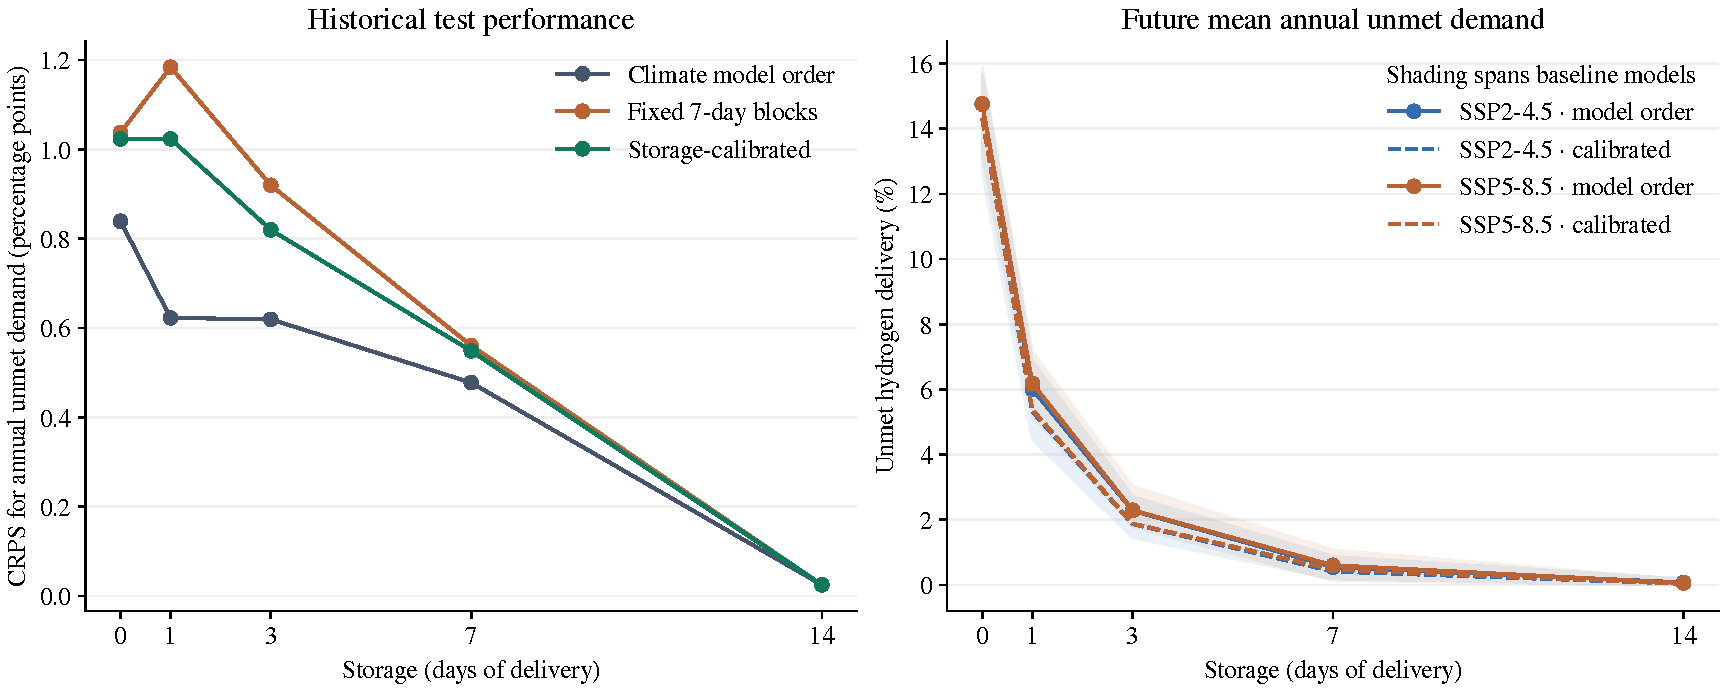
\includegraphics[width=\linewidth]{figures/hydrogen.pdf}
\caption{Historical test CRPS and projected mean annual unmet demand by tank size. The future panel shows 2041--2060 means. Solid lines retain climate-model order, dashed lines use storage-calibrated rank blocks, and shading spans the three baseline model means. Lower historical CRPS indicates better distributional agreement with the ERA5 reference.}
\label{fig:hydrogen}
\end{figure}

\clearpage
\begin{figure}[H]
\centering
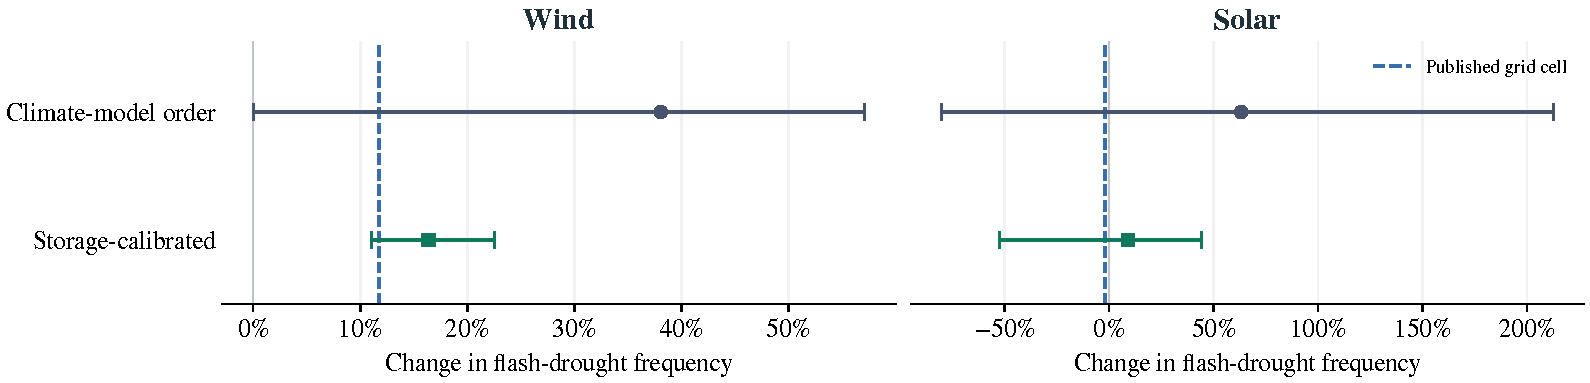
\includegraphics[width=.94\linewidth]{figures/flash-droughts.pdf}
\caption{Projected change in wind and solar flash-drought frequency under SSP2-4.5, comparing 2045--2074 with 1985--2014. Points show the pilot mean and horizontal intervals show the minimum and maximum across three models. The vertical marker in each panel shows the nearest eligible cell from the published Figure~2 workbook. The panels use separate horizontal scales.}
\label{fig:external}
\end{figure}

\section{Reproduction and data audit}
\label{app:reproduction}
The \RepoRoot\ provides the source, study configuration, and public-input retrieval code. To reproduce the experiment and the published-data comparison, use the benchmark branch, install the locked Python 3.12 dependencies and the workbook reader, then run the following commands from the repository root.

\begin{verbatim}
python -m beyond_normal.data all
python -m beyond_normal.run
python -m beyond_normal.benchmark --download
python -m beyond_normal.data cmip6 --future-years 2045 2074 \
  --experiments ssp245 --output data/raw/lin-2026
python -m beyond_normal.benchmark
python -m unittest discover -s tests -v
\end{verbatim}

The \RepoBenchmarks\ pin the results at commit \href{\RepoURL/commit/83839f69de4a26d76416b49299778d05279e79ef}{\texttt{83839f6}}. The \href{\RepoURL/blob/hydrogen-benchmarks/study.toml}{study configuration} records the plant, periods, scenario settings, and random seed. The \href{\RepoURL/blob/hydrogen-benchmarks/data/source/cmip6_stores.csv}{pinned CMIP6 catalog} records the exact realization, grid, version, and source URL. The \href{\RepoURL/blob/hydrogen-benchmarks/reports/run_manifest.json}{pipeline manifest} lists input and configuration checksums, software versions, and the selected parameters. The \href{\RepoURL/blob/hydrogen-benchmarks/reports/flash_drought_manifest.json}{external comparison manifest} specifies the grid cell, input periods, and checksum of the source workbook archive. The \href{\RepoURL/blob/hydrogen-benchmarks/reports/flash_drought_model_comparison.csv}{model-level counts} allow the published comparison to be audited before averaging.


\end{document}
